%%
%
% ARQUIVO: apendice.tex
%
% VERSÃO: 1.0
% DATA: Maio de 2016
% AUTOR: Coordenação de Trabalhos Especiais SE/8
% 
%  Arquivo tex de exemplo de apêndice do documento de Projeto de Fim de Curso.
%  Este exemplo traz dois apêndices (dois comandos \chapter{•}). Poderiam ser colocados em arquivos .tex
%  separados. Neste caso, o arquivo main.tex deveria ter um \include{•} para cada arquivo .tex
%
% ---
% DETALHES
%  a. todo apêndice deve começar com \chapter{•}
%  b. usar comando \noindent logo após \chapter{•}
%  c. segue os mesmos DETALHES do arquivo .tex de exemplo de capítulo do documento de Projeto de Fim de Curso
% ---
%%


\chapter{Apêndice}
\noindent


\section{Configurações Receptor via porta serial no BNC}

\begin{figure}[H]
\centering
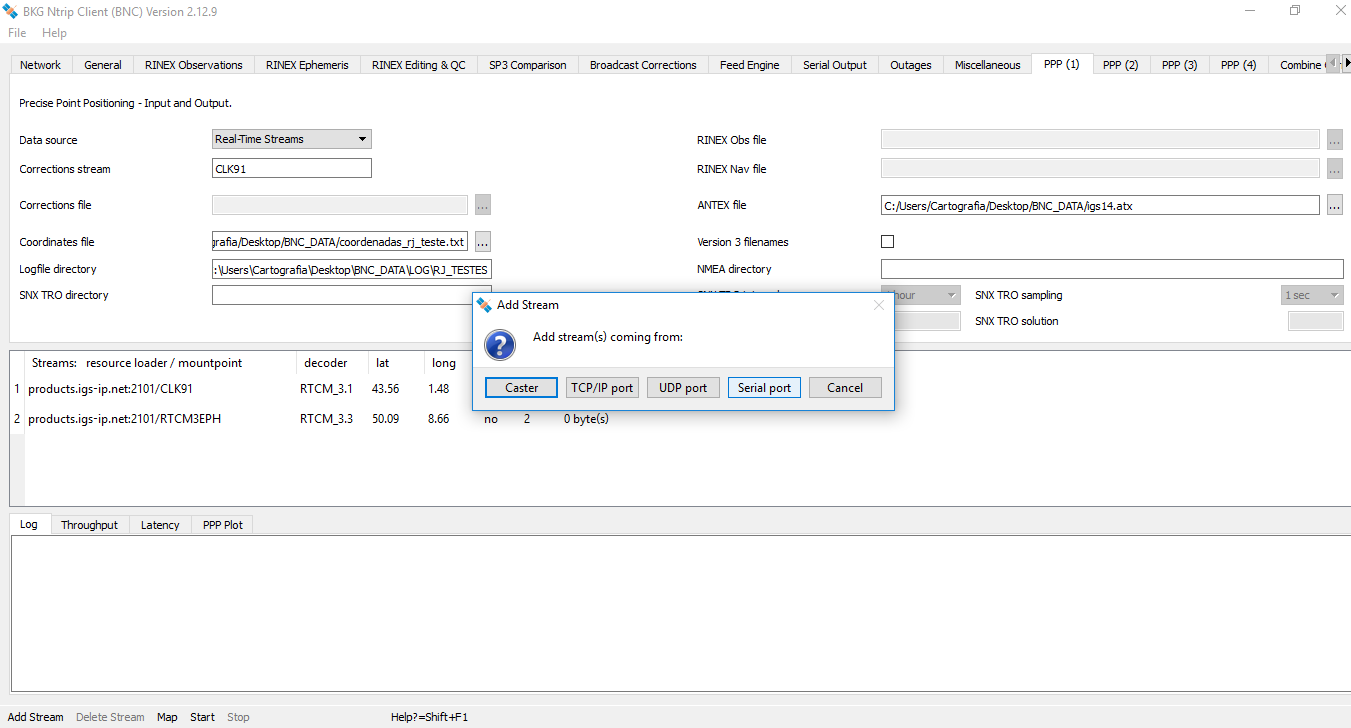
\includegraphics[scale=0.4]{img/18bnc.png} %scale eh o tamanho que a figura vai ficar
\caption{Seleção do receptor como Caster via portal serial.}
\label{Rotulo}
\end{figure}


\begin{figure}[H]
\centering
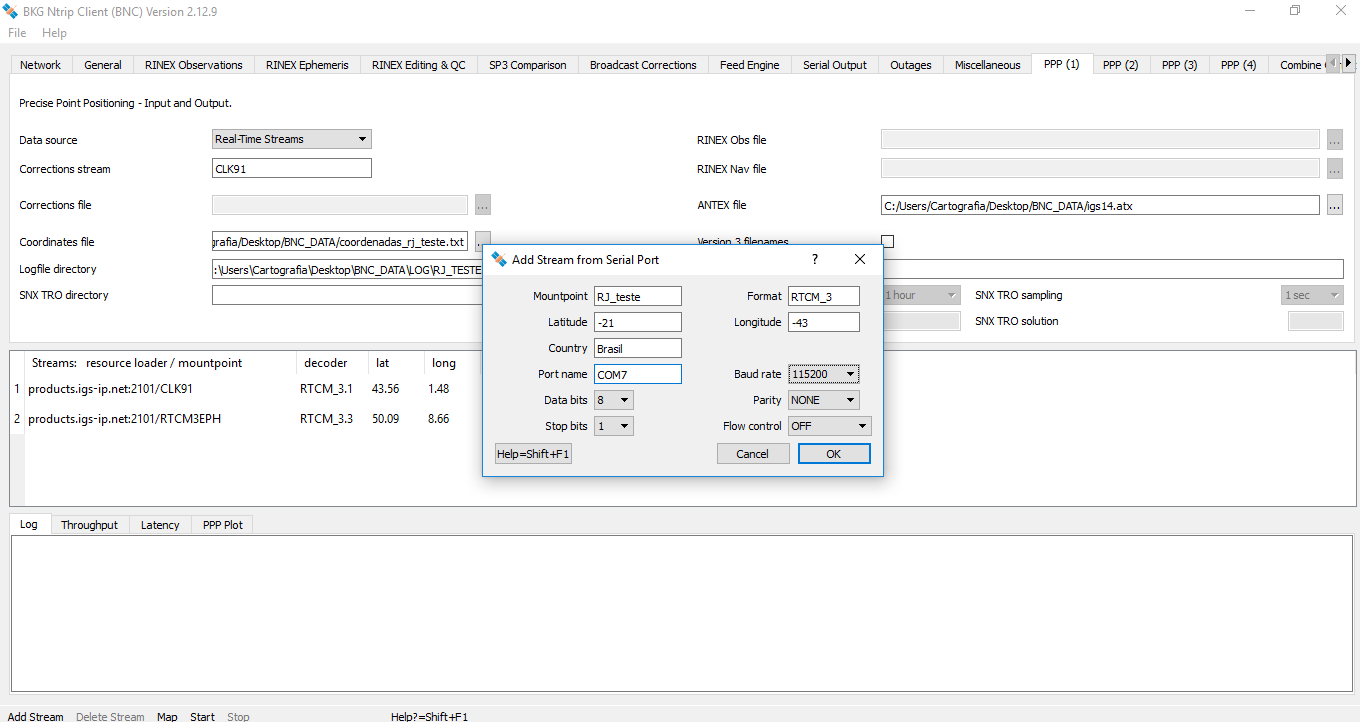
\includegraphics[scale=0.4]{img/19bnc.png} %scale eh o tamanho que a figura vai ficar
\caption{Configurações do receptor.}
\label{Rotulo}
\end{figure}


\begin{figure}[H]
\centering
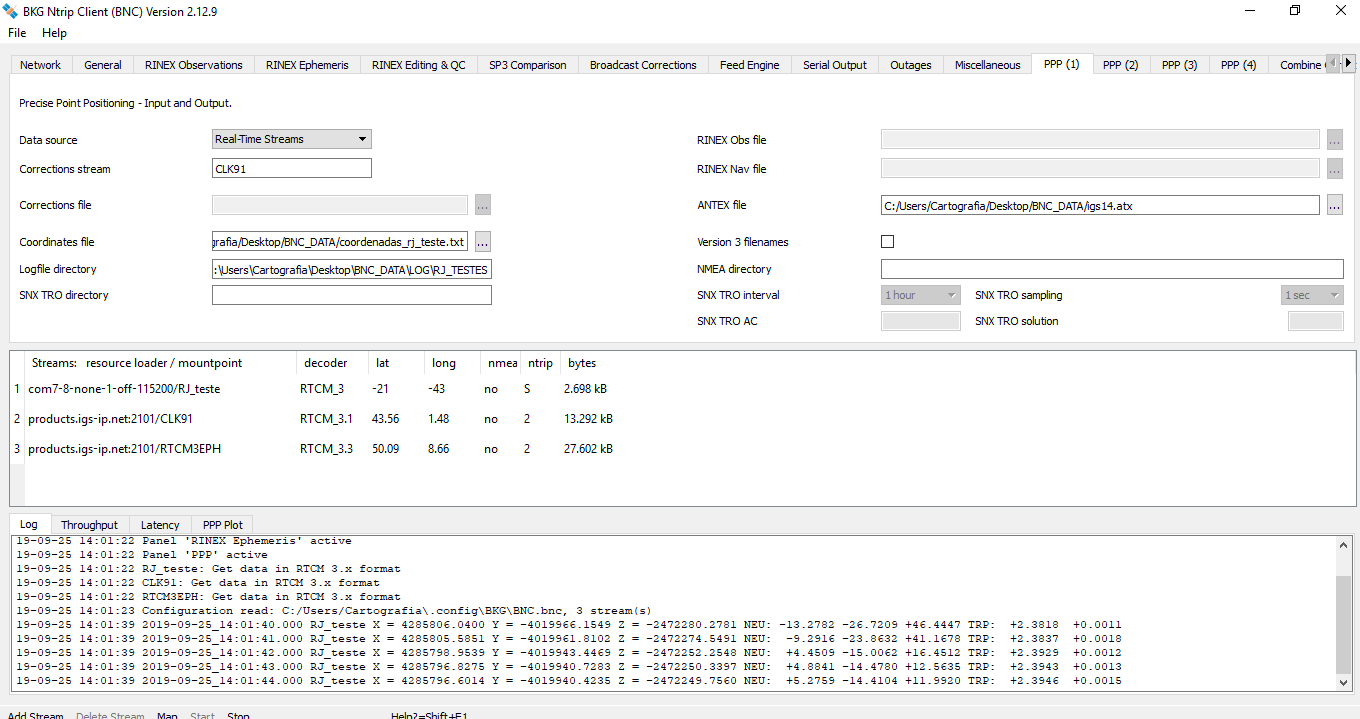
\includegraphics[scale=0.4]{img/21bnc.png} %scale eh o tamanho que a figura vai ficar
\caption{Chegada de dados do receptor para o BNC.}
\label{Rotulo}
\end{figure}






\section{Configurações de comunicação entre Receptor e Notebook via software TRU}

\begin{figure}[H]
\centering
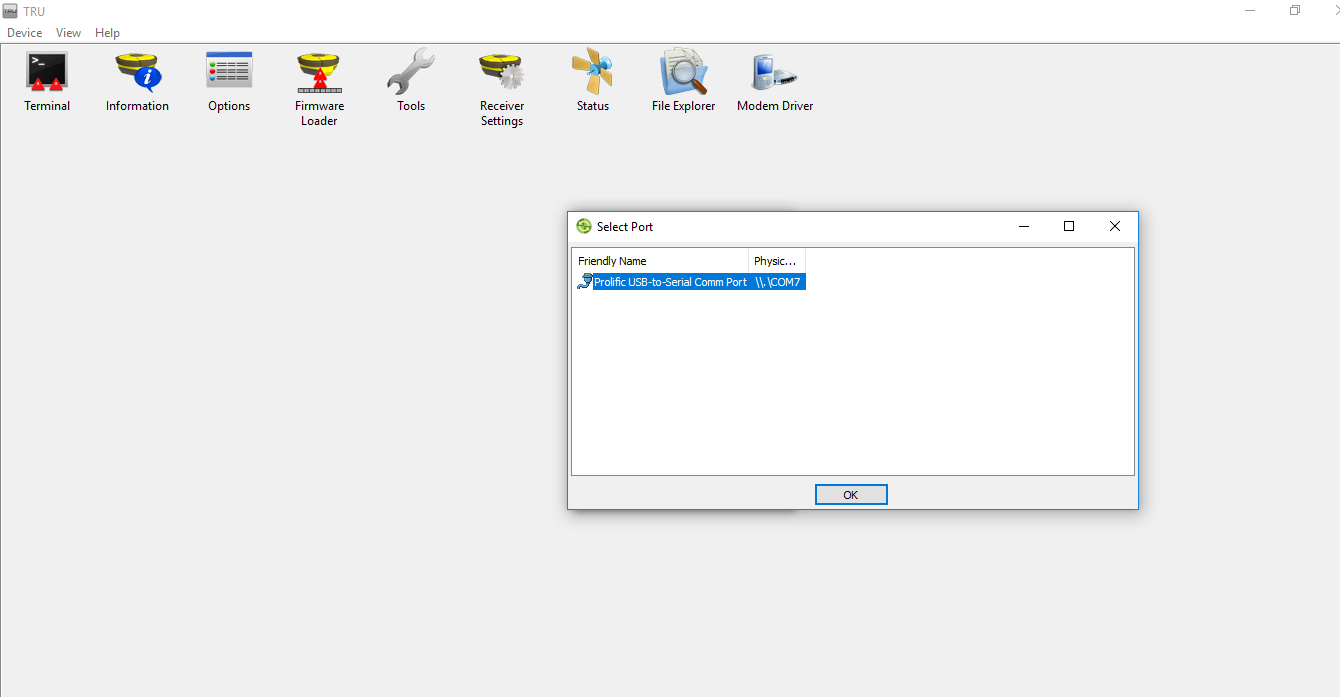
\includegraphics[scale=0.4]{img/2.png} %scale eh o tamanho que a figura vai ficar
\caption{Identificação da conexão do receptor via porta serial.}
\label{Rotulo}
\end{figure}


\begin{figure}[H]
\centering
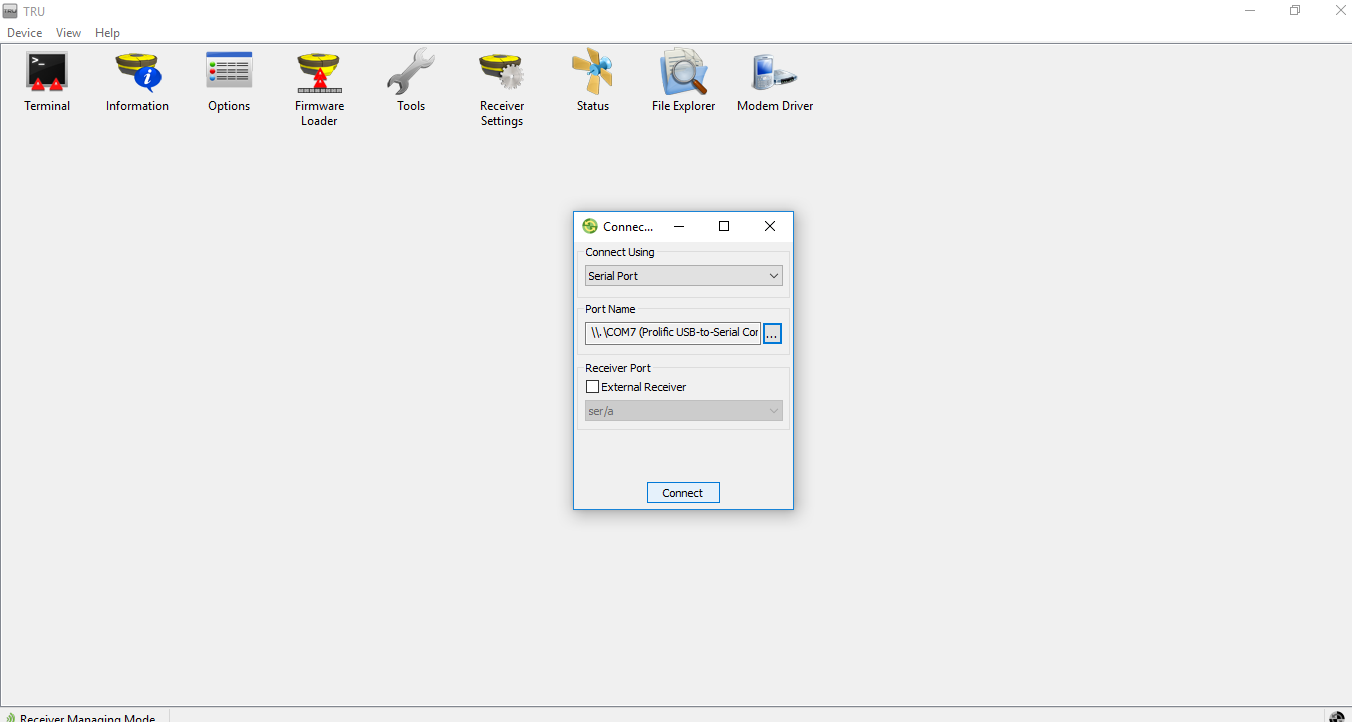
\includegraphics[scale=0.4]{img/3.png} %scale eh o tamanho que a figura vai ficar
\caption{Seleção e atribuição da porta serial ao receptor e conexão.}
\label{Rotulo}
\end{figure}


\begin{figure}[H]
\centering
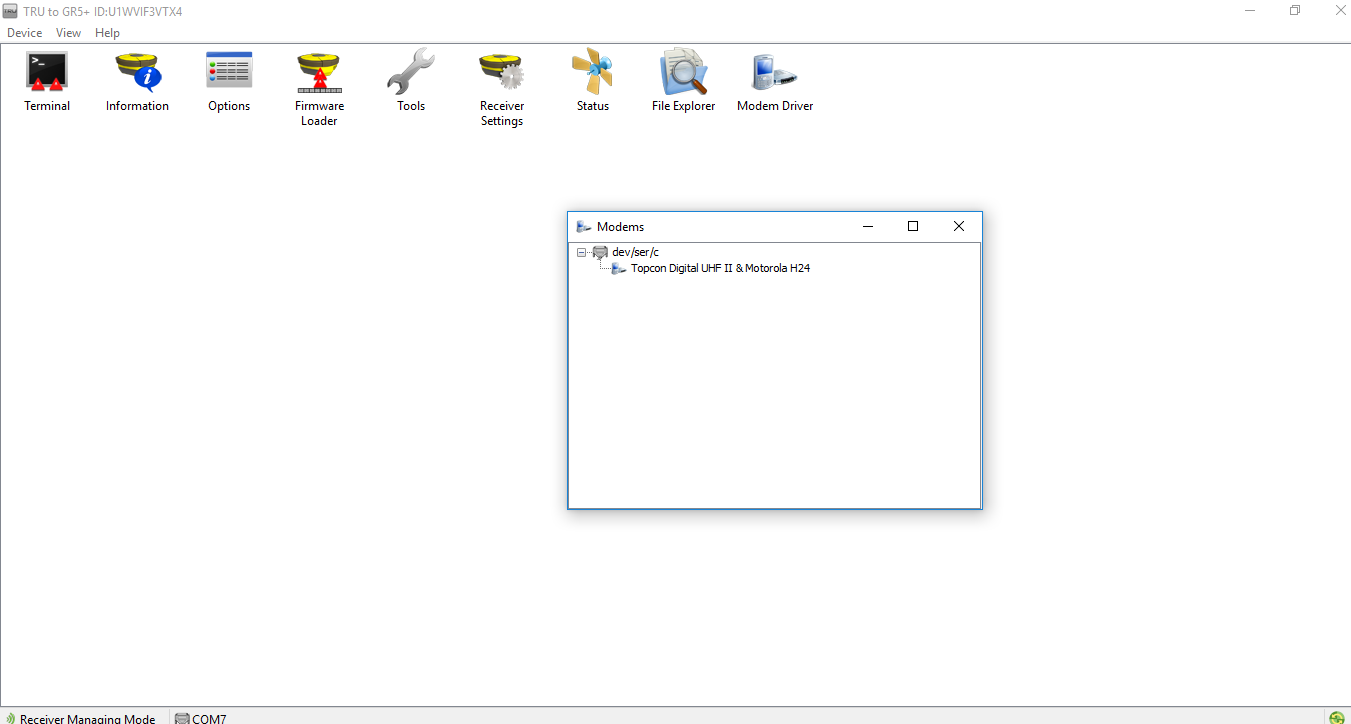
\includegraphics[scale=0.4]{img/4.png} %scale eh o tamanho que a figura vai ficar
\caption{Configurações de drivers.}
\label{Rotulo}
\end{figure}


\begin{figure}[H]
\centering
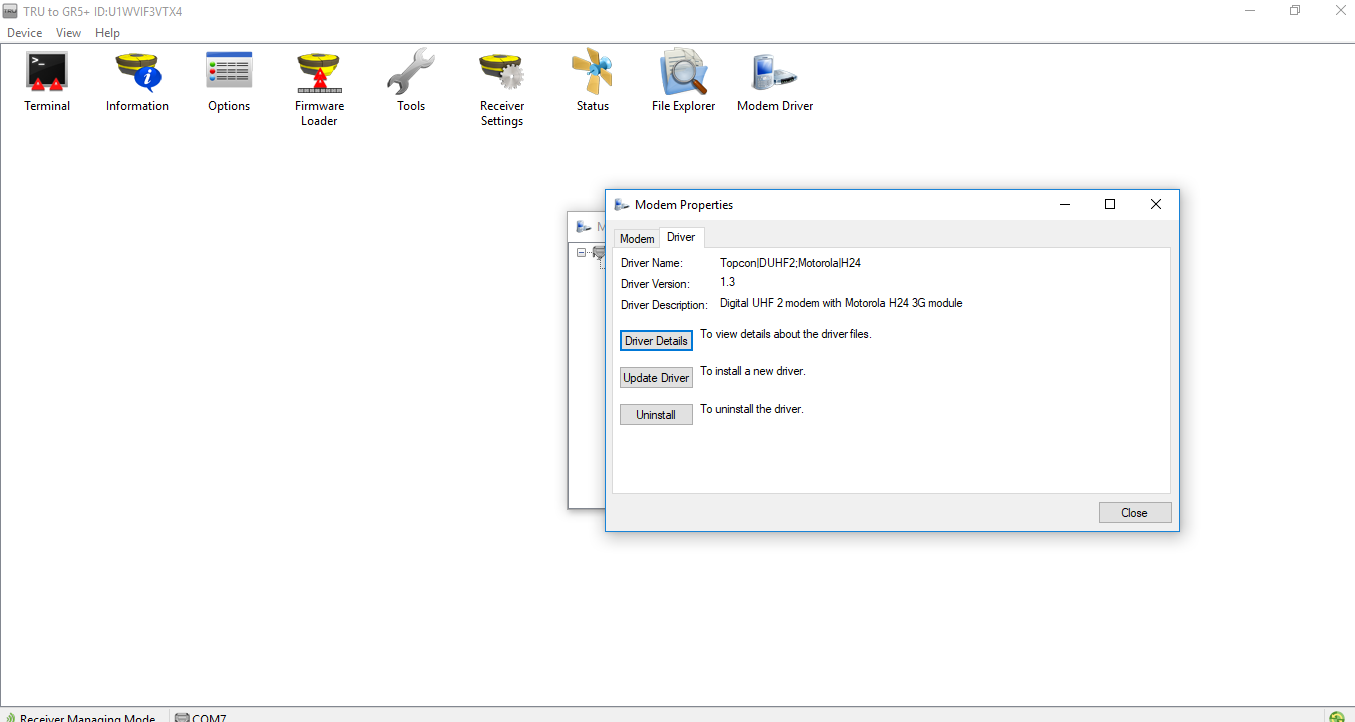
\includegraphics[scale=0.4]{img/5.png} %scale eh o tamanho que a figura vai ficar
\caption{Atualização de drivers}
\label{Rotulo}
\end{figure}

\begin{figure}[H]
\centering
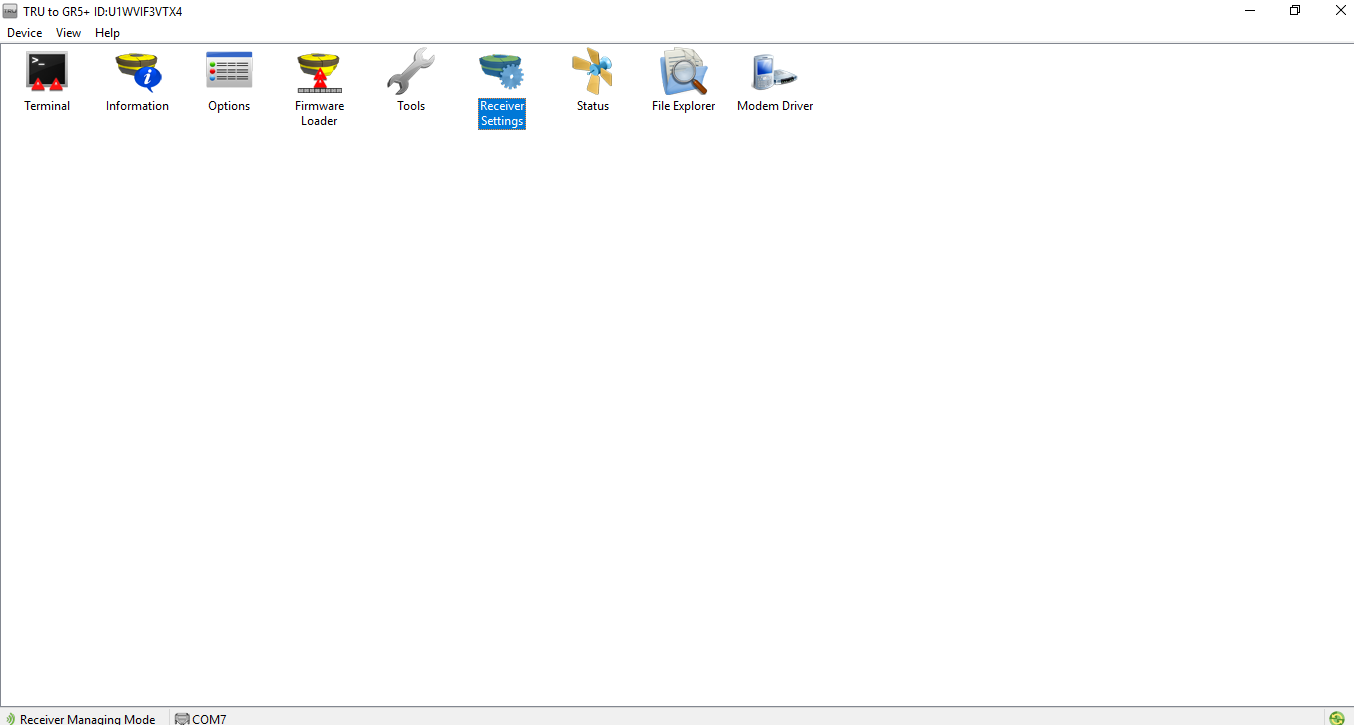
\includegraphics[scale=0.4]{img/6.png} %scale eh o tamanho que a figura vai ficar
\caption{Configurações do receptor.}
\label{Rotulo}
\end{figure}


\begin{figure}[H]
\centering
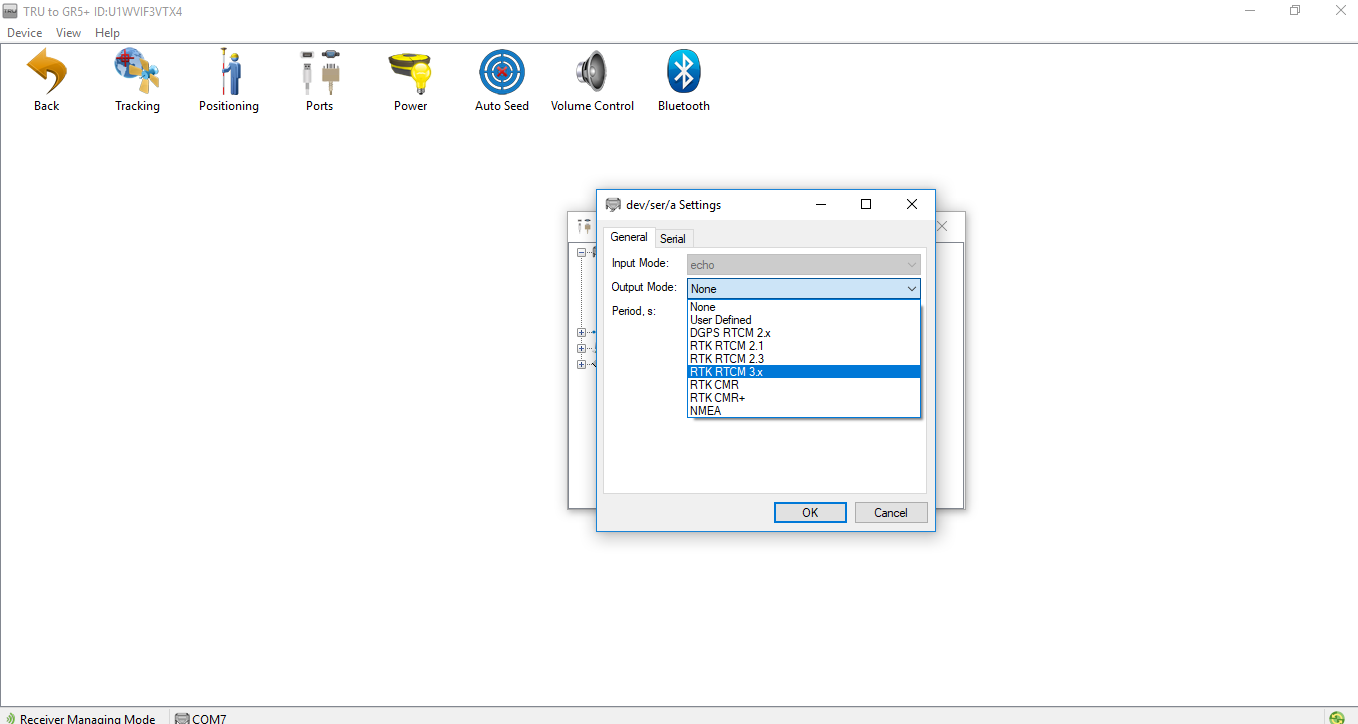
\includegraphics[scale=0.4]{img/9.png} %scale eh o tamanho que a figura vai ficar
\caption{Formato dos dados de saída.}
\label{Rotulo}
\end{figure}

\begin{figure}[H]
\centering
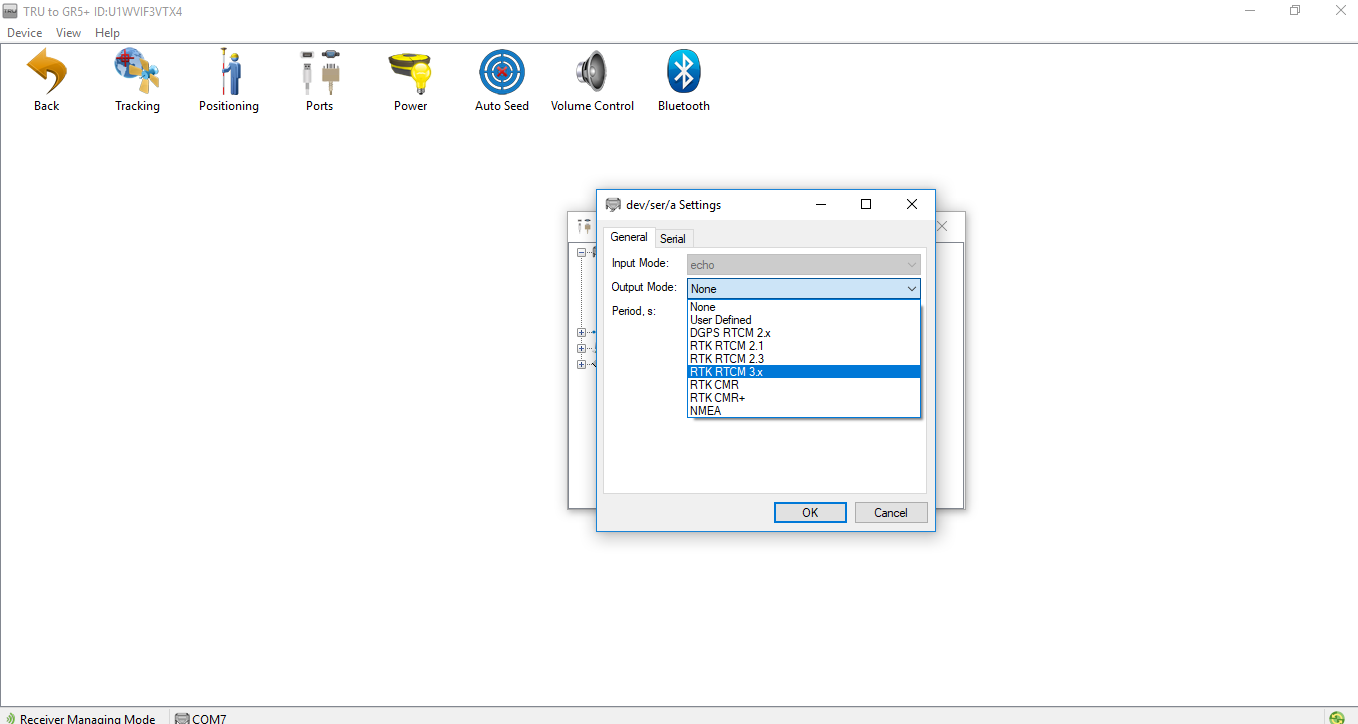
\includegraphics[scale=0.4]{img/9.png} %scale eh o tamanho que a figura vai ficar
\caption{Configuração de Baud Rate, Byte Size, Stop Bits e Parity.}
\label{Rotulo}
\end{figure}


\begin{figure}[H]
\centering
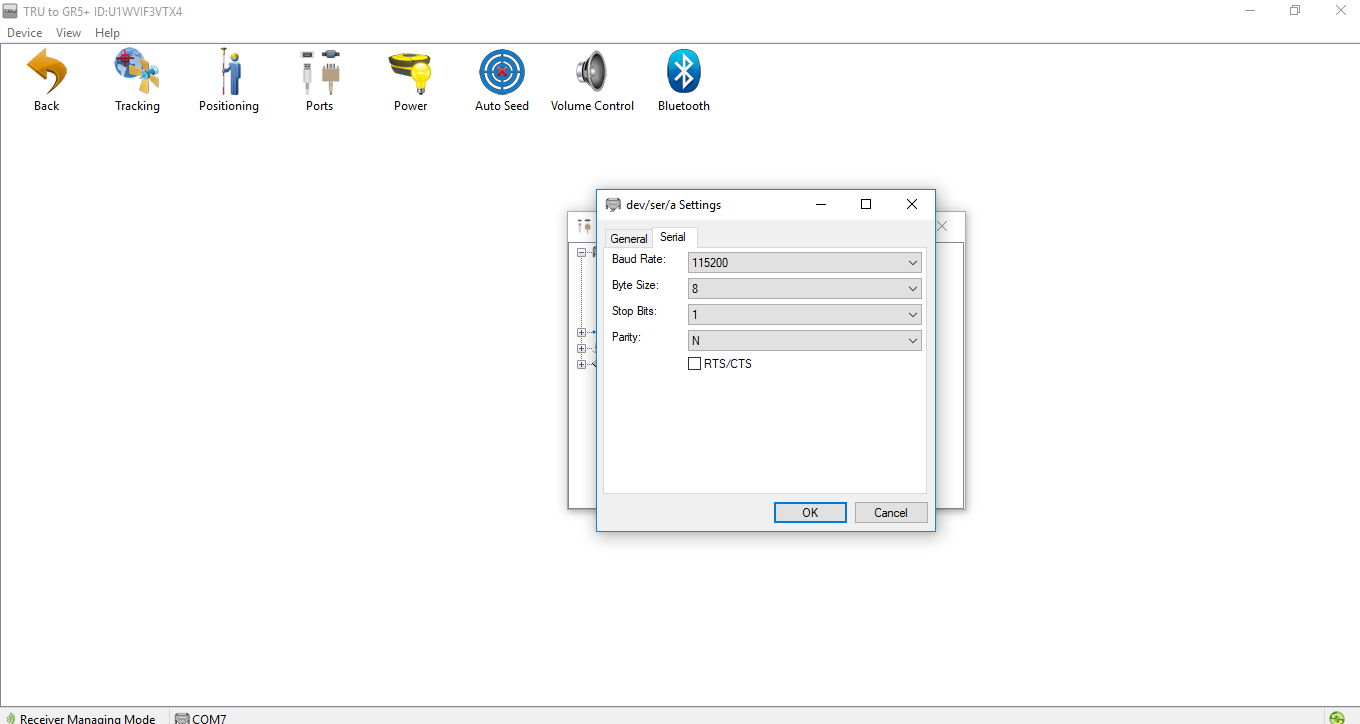
\includegraphics[scale=0.4]{img/11.png} %scale eh o tamanho que a figura vai ficar
\caption{Configuração de Baud Rate, Byte Size, Stop Bits e Parity.}
\label{Rotulo}
\end{figure}

\begin{figure}[H]
\centering
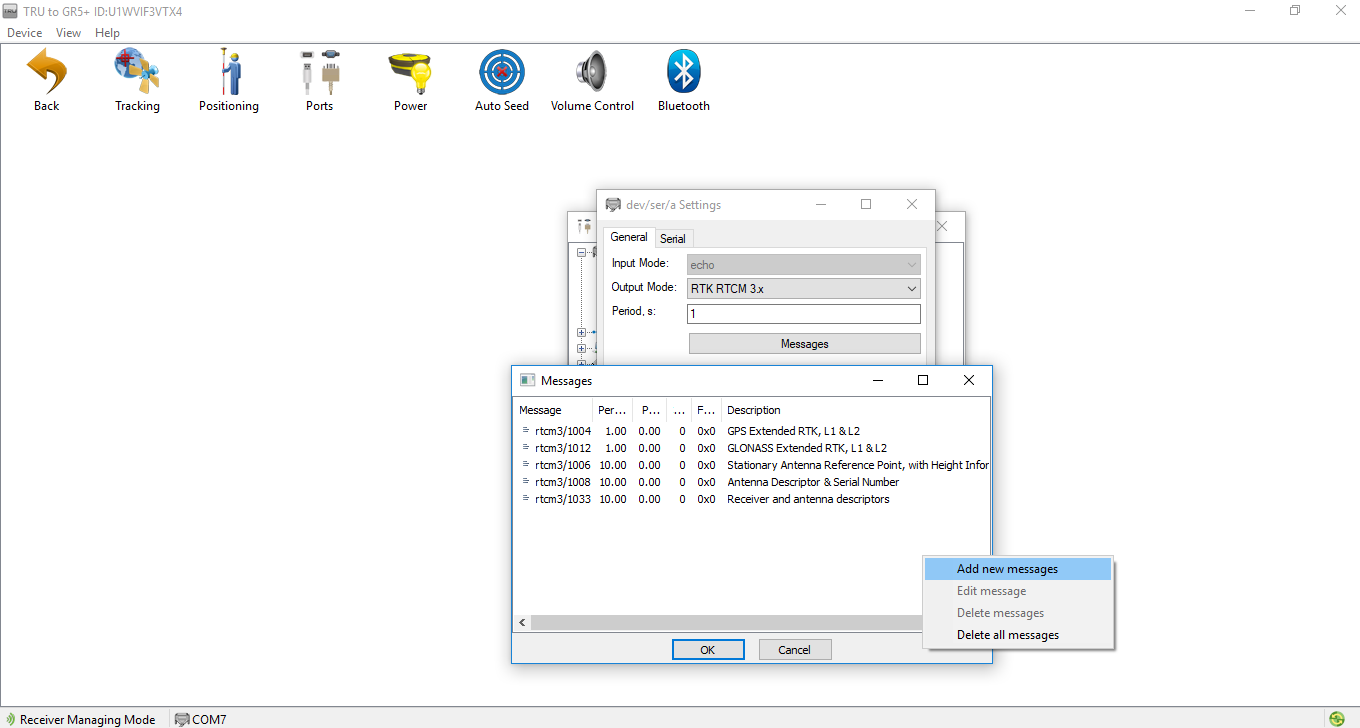
\includegraphics[scale=0.4]{img/13.png} %scale eh o tamanho que a figura vai ficar
\caption{Seleção das mensagens de chegada no receptor.}
\label{Rotulo}
\end{figure}

\begin{figure}[H]
\centering
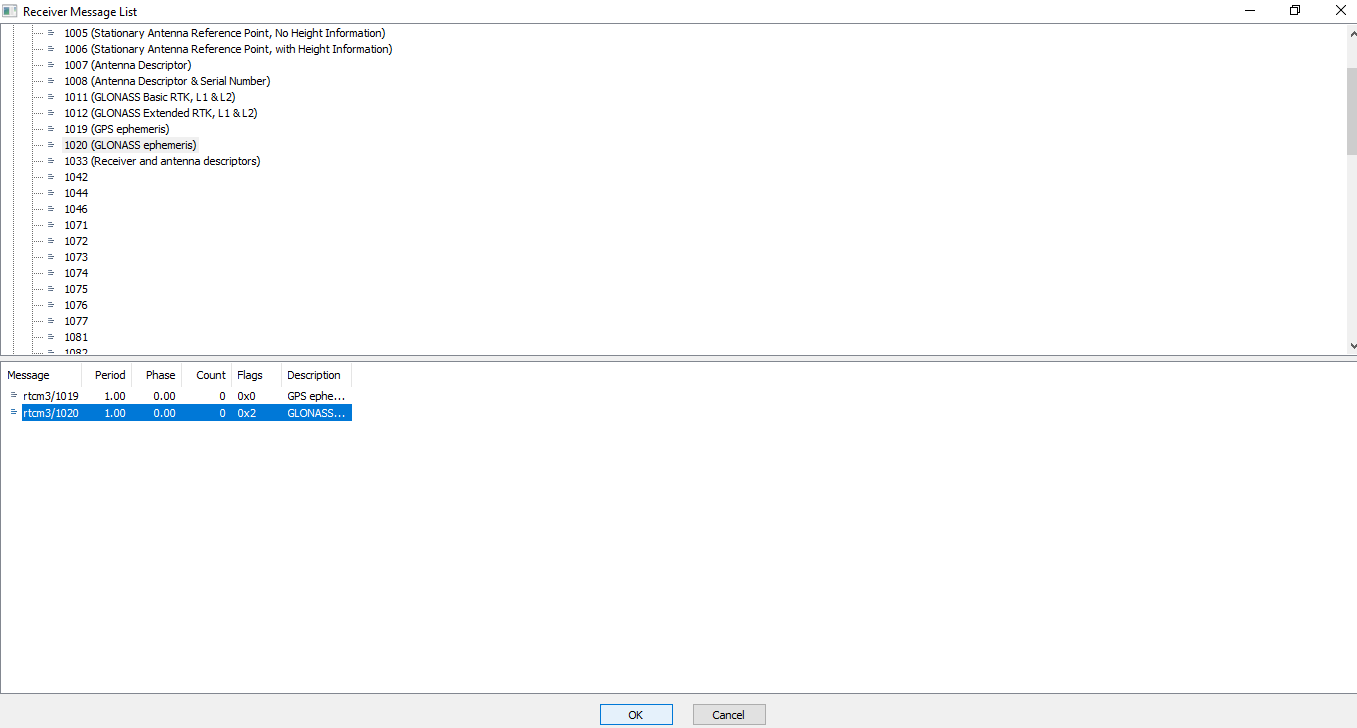
\includegraphics[scale=0.4]{img/14.png} %scale eh o tamanho que a figura vai ficar
\caption{Seleção das mensagens de chegada no receptor.}
\label{Rotulo}
\end{figure}

\begin{figure}[H]
\centering
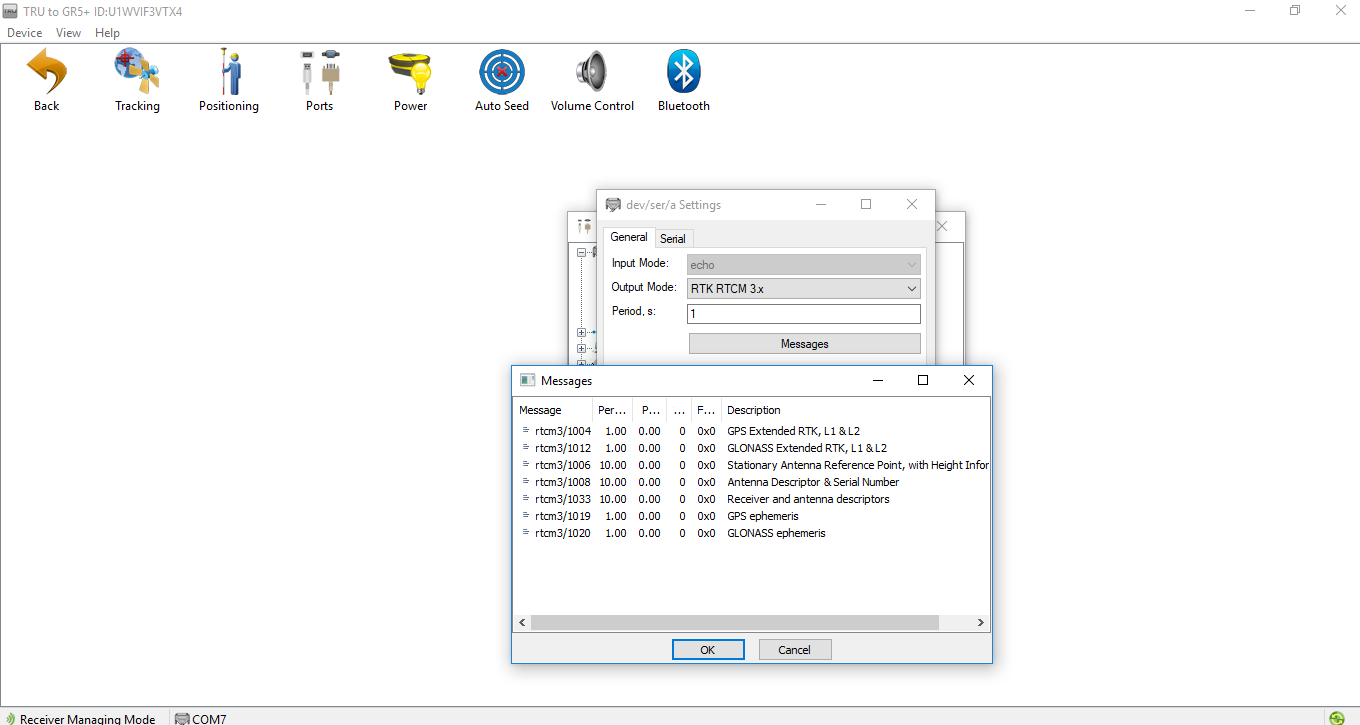
\includegraphics[scale=0.4]{img/15.png} %scale eh o tamanho que a figura vai ficar
\caption{Seleção das mensagens de chegada no receptor.}
\label{Rotulo}
\end{figure}

\begin{figure}[H]
\centering
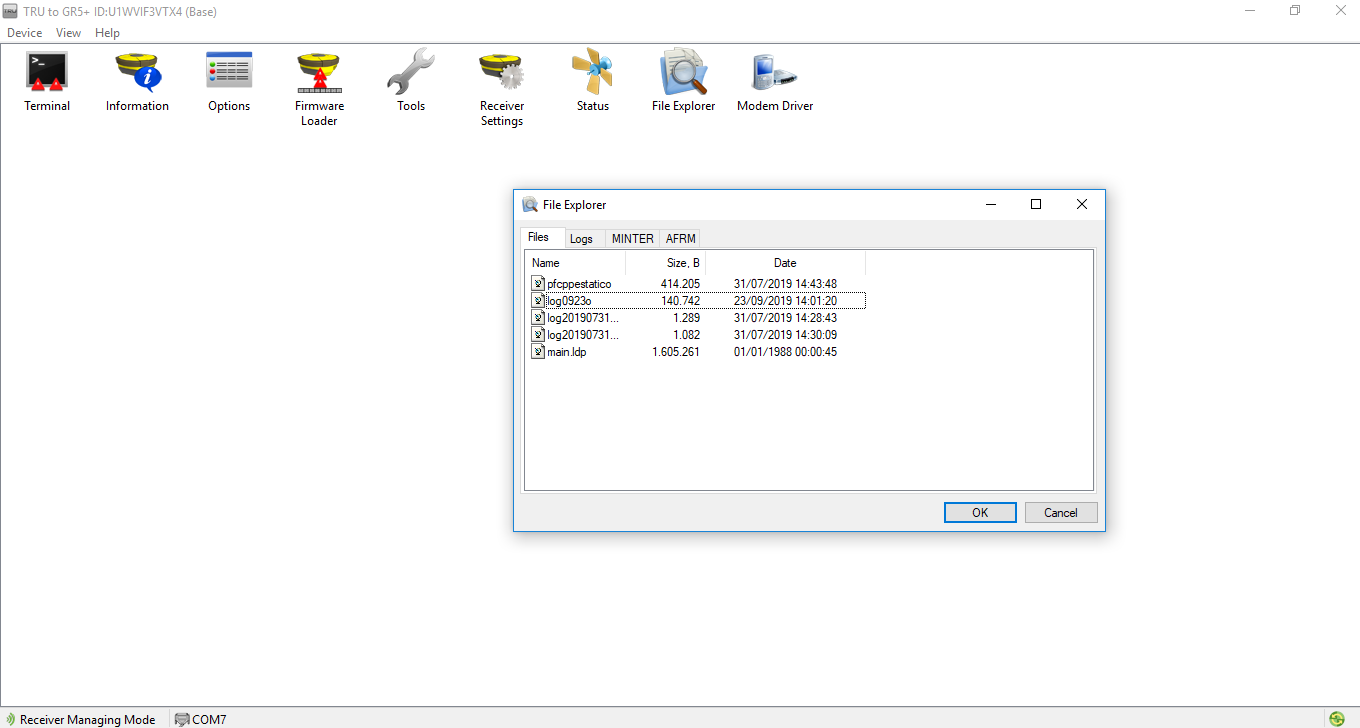
\includegraphics[scale=0.4]{img/17.png} %scale eh o tamanho que a figura vai ficar
\caption{ Visualização de arquivos log.}
\label{Rotulo}
\end{figure}


\section{Códigos construídos (Python3) para extração de dados do RTPPP e exibição de gráficos}
\subsection{Código ''main.py''}
\lstinputlisting{data/main.py}

\subsection{Funções auxiliares}
\lstinputlisting{data/graphics.py}

\subsection{Funções para construção dos gráficos e extração dos dados}
\lstinputlisting{data/auxiliary_functions.py}


\section{Extrato do LOG obtido no BNC 2.12 ao realizar RTPPP na estação POAL}

\begin{lstlisting}
19-07-27 00:00:23 2019-07-27_00:00:10.000 POAL00BRA0 X = 3467519.3895 Y = -4300378.7366 Z = -3177517.5357 NEU:  +0.2430  -0.1367  +0.0316 TRP:  +2.3821  +0.0336
19-07-27 00:00:23 2019-07-27_00:00:11.000 POAL00BRA0 X = 3467519.3976 Y = -4300378.7418 Z = -3177517.5480 NEU:  +0.2369  -0.1336  +0.0458 TRP:  +2.3821  +0.0336
19-07-27 00:00:23 2019-07-27_00:00:12.000 POAL00BRA0 X = 3467519.3928 Y = -4300378.7414 Z = -3177517.5469 NEU:  +0.2361  -0.1372  +0.0423 TRP:  +2.3821  +0.0336
19-07-27 00:00:23 2019-07-27_00:00:13.000 POAL00BRA0 X = 3467519.3987 Y = -4300378.7494 Z = -3177517.5474 NEU:  +0.2407  -0.1375  +0.0511 TRP:  +2.3821  +0.0336
19-07-27 00:00:23 2019-07-27_00:00:14.000 POAL00BRA0 X = 3467519.3960 Y = -4300378.7405 Z = -3177517.5460 NEU:  +0.2376  -0.1341  +0.0429 TRP:  +2.3821  +0.0336
19-07-27 00:00:29 2019-07-27_00:00:15.000 POAL00BRA0 X = 3467519.3999 Y = -4300378.7434 Z = -3177517.5477 NEU:  +0.2385  -0.1329  +0.0479 TRP:  +2.3821  +0.0336
19-07-27 00:00:29 2019-07-27_00:00:16.000 POAL00BRA0 X = 3467519.3985 Y = -4300378.7423 Z = -3177517.5495 NEU:  +0.2361  -0.1332  +0.0473 TRP:  +2.3821  +0.0336
19-07-27 00:00:29 2019-07-27_00:00:17.000 POAL00BRA0 X = 3467519.4080 Y = -4300378.7514 Z = -3177517.5514 NEU:  +0.2410  -0.1316  +0.0595 TRP:  +2.3821  +0.0336
19-07-27 00:00:29 2019-07-27_00:00:18.000 POAL00BRA0 X = 3467519.4062 Y = -4300378.7469 Z = -3177517.5530 NEU:  +0.2373  -0.1302  +0.0564 TRP:  +2.3821  +0.0336
19-07-27 00:00:29 2019-07-27_00:00:19.000 POAL00BRA0 X = 3467519.3978 Y = -4300378.7404 Z = -3177517.5431 NEU:  +0.2406  -0.1326  +0.0424 TRP:  +2.3821  +0.0336
19-07-27 00:00:34 2019-07-27_00:00:20.000 POAL00BRA0 X = 3467519.3852 Y = -4300378.7235 Z = -3177517.5396 NEU:  +0.2331  -0.1318  +0.0224 TRP:  +2.3821  +0.0336
19-07-27 00:00:34 2019-07-27_00:00:21.000 POAL00BRA0 X = 3467519.3970 Y = -4300378.7415 Z = -3177517.5496 NEU:  +0.2352  -0.1339  +0.0460 TRP:  +2.3821  +0.0336
19-07-27 00:00:34 2019-07-27_00:00:22.000 POAL00BRA0 X = 3467519.4080 Y = -4300378.7424 Z = -3177517.5555 NEU:  +0.2339  -0.1260  +0.0555 TRP:  +2.3821  +0.0336
19-07-27 00:00:34 2019-07-27_00:00:23.000 POAL00BRA0 X = 3467519.3999 Y = -4300378.7319 Z = -3177517.5484 NEU:  +0.2334  -0.1257  +0.0405 TRP:  +2.3821  +0.0336
19-07-27 00:00:34 2019-07-27_00:00:24.000 POAL00BRA0 X = 3467519.4032 Y = -4300378.7340 Z = -3177517.5499 NEU:  +0.2339  -0.1244  +0.0445 TRP:  +2.3821  +0.0336
19-07-27 00:00:38 2019-07-27_00:00:25.000 POAL00BRA0 X = 3467519.3932 Y = -4300378.7370 Z = -3177517.5502 NEU:  +0.2317  -0.1341  +0.0412 TRP:  +2.3821  +0.0336
19-07-27 00:00:38 2019-07-27_00:00:26.000 POAL00BRA0 X = 3467519.3946 Y = -4300378.7278 Z = -3177517.5459 NEU:  +0.2323  -0.1272  +0.0336 TRP:  +2.3821  +0.0336
19-07-27 00:00:38 2019-07-27_00:00:27.000 POAL00BRA0 X = 3467519.3969 Y = -4300378.7290 Z = -3177517.5462 NEU:  +0.2333  -0.1261  +0.0358 TRP:  +2.3821  +0.0335
19-07-27 00:00:38 2019-07-27_00:00:28.000 POAL00BRA0 X = 3467519.4109 Y = -4300378.7383 Z = -3177517.5521 NEU:  +0.2362  -0.1211  +0.0526 TRP:  +2.3821  +0.0335
19-07-27 00:00:38 2019-07-27_00:00:29.000 POAL00BRA0 X = 3467519.4076 Y = -4300378.7349 Z = -3177517.5535 NEU:  +0.2326  -0.1216  +0.0493 TRP:  +2.3821  +0.0335
19-07-27 00:00:43 2019-07-27_00:00:30.000 POAL00BRA0 X = 3467519.3959 Y = -4300378.7388 Z = -3177517.5452 NEU:  +0.2377  -0.1331  +0.0414 TRP:  +2.3821  +0.0335
\end{lstlisting}
\section{Arquivo de coordenadas da estação POAL para realização de RTPPP com software BNC}
\begin{lstlisting}
        POAL00BRA0  3467519.4343  -4300378.65881  -3177517.52227  0.0000  0.0000  0.0010 TRM115000.00    NONE TRIMBLE NETR9
 \end{lstlisting}